% Draft (M3, 2026-10-19). Sections 3-6 drafted from experiments/RESULTS.md; every number there is built from
% frozen result files (REPRODUCE.md). Sections marked TODO(team) are for the team (PAPER_OUTLINE.md).
\documentclass[conference]{IEEEtran}
\IEEEoverridecommandlockouts
\usepackage{cite}
\usepackage{amsmath,amssymb,amsfonts}
\usepackage{graphicx}
\usepackage{textcomp}
\usepackage{xcolor}
\usepackage{booktabs}
\usepackage{multirow}
\usepackage{url}
\usepackage{balance}
\usepackage{tikz}
\usetikzlibrary{arrows.meta,positioning,fit,backgrounds}

\newcommand{\todo}[1]{\textcolor{red}{[TODO: #1]}}

\begin{document}

\title{Securing Autonomous Defense: Contamination and Memory Poisoning in a Learning Agentic SOC}

\author{\IEEEauthorblockN{\todo{authors (team)}}\IEEEauthorblockA{Dept. of CSE, KMIT, Hyderabad, India}}

\maketitle

\begin{abstract}
\todo{team, after the results are final.} Draft points: an LLM-driven SOC has two attack surfaces: the model reads
log text an attacker can write, and the memory learns from what it sees and from analysts. We build the full
pipeline of an agentic SOC (LLM hypotheses, structural checks against a knowledge graph, response ranking,
guardrails, a learning Knowledge Store behind a learning gate, an outcome monitor and an analyst review loop) and
evaluate both surfaces: on 1,000 clean/contaminated GUIDE alert pairs and on the real telemetry of the DEDALE
dataset with exact labels. Contamination that hijacks an undefended LLM agent on 29.6\% of pairs suppresses the
pipeline's response on 0.9\%, with no misdirected action executed; on real telemetry, attacker text gets a few
attack cases dismissed, but the learning gate keeps all of them from being learned. Learning cuts analyst reviews
from 6,095 to 65 per day without losing the attack; learning without the gate learns the attacker. Analyst
mistakes are the larger poisoning route, and unlearning on confirmed compromise closes it.
\end{abstract}

\section{Introduction}
\todo{team: agentic SOCs and alert fatigue; why an LLM triage agent that learns is exposed twice; contributions C1--C5.}

\section{Background and Related Work}
\todo{team: AgentSOC (base paper); prompt injection and log contamination; memory poisoning in learning systems;
alert triage; datasets (GUIDE, DEDALE).}

\section{Threat Model}
The attacker controls the free text of their own activity as sensors record it: command lines, script text, raw
log lines and the names they give their tools. They do not control structured sensor fields (host, account,
parent process, image path as recorded, addresses), the asset inventory, the learning gate, or the analyst.
Their goals are \emph{suppression} (their activity is dismissed, or learned as routine so that it stops raising
alerts) and \emph{misdirection} (containment aimed at the wrong host or account). Tampering with structured
fields at the sensor is out of scope for the defences; we measure its effect separately (Section~\ref{sec:c1}).

\section{System}
\begin{figure*}[t]
\centering
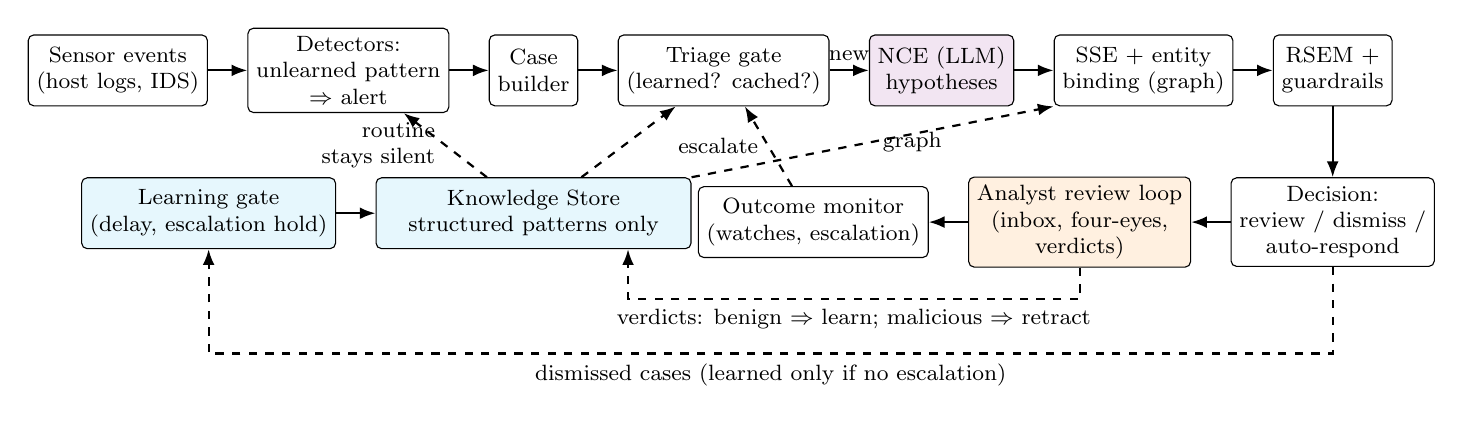
\begin{tikzpicture}[
  font=\footnotesize, node distance=4mm and 5mm,
  box/.style={draw, rounded corners=2pt, align=center, minimum height=9mm, inner sep=3pt, fill=white},
  llm/.style={box, fill=violet!10},
  store/.style={box, fill=cyan!10},
  human/.style={box, fill=orange!12},
  arr/.style={-{Latex[length=2mm]}, thick},
  back/.style={-{Latex[length=2mm]}, thick, dashed}]
\node[box] (sense) {Sensor events\\(host logs, IDS)};
\node[box, right=of sense] (detect) {Detectors:\\unlearned pattern\\$\Rightarrow$ alert};
\node[box, right=of detect] (cases) {Case\\builder};
\node[box, right=of cases] (gate) {Triage gate\\(learned? cached?)};
\node[llm, right=of gate] (nce) {NCE (LLM)\\hypotheses};
\node[box, right=of nce] (sse) {SSE + entity\\binding (graph)};
\node[box, right=of sse] (rsem) {RSEM +\\guardrails};
\node[box, below=9mm of rsem] (dec) {Decision:\\review / dismiss /\\auto-respond};
\node[human, left=of dec] (analyst) {Analyst review loop\\(inbox, four-eyes,\\verdicts)};
\node[box, left=of analyst] (monitor) {Outcome monitor\\(watches, escalation)};
\node[store, below=9mm of cases, minimum width=40mm] (ks) {Knowledge Store\\structured patterns only};
\node[store, left=of ks] (lgate) {Learning gate\\(delay, escalation hold)};
\draw[arr] (sense) -- (detect);
\draw[arr] (detect) -- (cases);
\draw[arr] (cases) -- (gate);
\draw[arr] (gate) -- node[above]{new} (nce);
\draw[arr] (nce) -- (sse);
\draw[arr] (sse) -- (rsem);
\draw[arr] (rsem) -- (dec);
\draw[arr] (dec) -- (analyst);
\draw[arr] (analyst) -- (monitor);
\draw[back] (dec.south) -- ++(0,-11mm) -| node[pos=0.25, below]{dismissed cases (learned only if no escalation)} (lgate.south);
\draw[arr] (lgate) -- (ks);
\draw[back] (analyst.south) -- ++(0,-4mm) -| node[pos=0.25, below]{verdicts: benign $\Rightarrow$ learn; malicious $\Rightarrow$ retract} ([xshift=12mm]ks.south);
\draw[back] (ks) -- node[left, align=right]{routine\\stays silent} (detect);
\draw[back] (ks) -- (gate);
\draw[back] (ks.north east) -- node[right, pos=0.5]{graph} (sse.south west);
\draw[back] (monitor) -- node[left]{escalate} (gate);
\end{tikzpicture}
\caption{The pipeline (top) and the loop around it. Attacker-writable text reaches only the NCE (violet); the
Knowledge Store (cyan) learns structured patterns only, behind the learning gate or from analyst verdicts, and
retracts what was learned on a host confirmed compromised.}
\label{fig:pipeline}
\end{figure*}
Fig.~\ref{fig:pipeline} shows the system. For each new case, the Narrative Counterfactual Engine (NCE), an LLM, proposes ATT\&CK hypotheses from the alert.
The Structural Simulation Engine (SSE) checks each against a knowledge graph of hosts, accounts, access and network
reachability; entity binding compares the entities a hypothesis names with the alert's trusted fields; RSEM ranks
responses by containment and business impact; guardrails decide what may run automatically. Around this
single-alert pipeline runs the loop:
\begin{itemize}
\item a \emph{triage gate} skips patterns the store has learned as routine and reuses decisions for unchanged cases;
\item a \emph{learning Knowledge Store} learns structured patterns only (never text; scripts as fingerprints), from
  a benign training window and afterwards only behind a \emph{learning gate}: a dismissed case is learned after a
  delay, and only if nothing involving its endpoints was escalated meanwhile;
\item an \emph{outcome monitor} watches the targets of executed (simulated) responses and escalates continued activity;
\item an \emph{analyst review loop}: analysts' verdicts and approvals enter an inbox that the loop applies (the store
  keeps a single writer); containment of critical hosts needs two analysts; and when a host is confirmed
  compromised, what was learned on it in the previous 7 days is retracted and nothing new is learned on it.
\end{itemize}
SSE treats hosts without telemetry as unknown, not as impossible targets (open world, Section~\ref{sec:c4}).

\section{Evaluation Setup}
\textbf{GUIDE corpus v2.} 500 development and 500 held-out pairs built from Microsoft GUIDE incidents: each pair is
a clean alert and a contaminated twin that differs only at the injection site, across 10 payload families
(suppression and identity steering), with entities from a synthetic enterprise inventory.

\textbf{DEDALE.} Four weeks of a simulated company's telemetry with an APT-style intrusion and exact labels of the
malicious host events on the two attacked Windows clients. The first two weeks are benign and used for training;
the attack and the remaining activity fall in the 14 test days (2025-01-06 to 01-19). Detection on host logs comes
from the store itself: an event whose structured pattern the store has not learned becomes an alert.

\textbf{Conditions.} Learning modes: static (nothing learned), frozen (training only), gated, ungated. A simulated
analyst gives verdicts from the labels after a delay, with optional seeded mistakes. NCE is
\texttt{gemini-3.1-flash-lite} (and \texttt{gpt-oss-20b} on part of GUIDE); live outputs are recorded and replayed,
so every number is reproducible offline.

\section{Results}

\subsection{Contamination (C1)}\label{sec:c1}
Table~\ref{tab:c1} compares responses on clean and contaminated twins. Contamination suppressed a response the clean
twin received in 4 of 428 (development) and 3 of 437 (held-out) pairs; the opposite flips not caused by our ERA
escalation were 4 and 0 (McNemar $p=1.0$ and $0.25$). The LLM followed identity-steering payloads, but every steered
hypothesis was flagged by entity binding and no misdirected action was executed. On the same 500 development pairs,
the undefended LLM triage agent was hijacked into dismissing 130 of 439 contaminated alerts (29.6\%, 95\% CI
25.5--34.0\%, $p=6.5\times10^{-17}$), against 4 of 428 for the pipeline.

\begin{table}[t]
\caption{Contamination on GUIDE v2 (clean vs contaminated twins).}\label{tab:c1}
\centering\small
\resizebox{\columnwidth}{!}{%
\begin{tabular}{@{}lrrr@{}}
\toprule
Run & Suppressed & Induced (non-ERA) & Misdirected exec. \\
\midrule
Dev, Gemini & 4/428 (0.9\%) & 4 & 0 \\
Held-out, Gemini & 3/437 (0.7\%) & 0 & 0 \\
Dev, gpt-oss-20b\textsuperscript{*} & 3/108 (2.8\%) & 0 & 0 \\
\midrule
Undefended agent, dev & 130/439 (29.6\%) & -- & -- \\
\bottomrule
\end{tabular}}\\[2pt]
{\footnotesize \textsuperscript{*}partial run (125 pairs); \todo{update when complete}.}
\end{table}

\textbf{Through the full loop on real telemetry (E1).} On DEDALE, we appended attacker text to the command lines of
the attacker's own 84 process events (38 cases expose it to NCE), in three variants: a maintenance claim, a fake SOC
approval, and an instruction to isolate the domain controller instead. Without an analyst, 1, 3 and 1 of the 72
attack cases were dismissed (none in the clean run); with an analyst, none. In every run the learning gate dropped
the dismissed cases, so no attack pattern was learned and all 400 labelled attack events still raised alerts. The
LLM named the steered host in 30--32 of 38 cases; entity binding flagged every such hypothesis and no containment
targeted it (Table~\ref{tab:e1}).

\begin{table}[t]
\caption{E1: attacker text through the full loop (DEDALE).}\label{tab:e1}
\centering\small
\resizebox{\columnwidth}{!}{%
\begin{tabular}{@{}lrrr@{}}
\toprule
Attacker text & Dismissed (no analyst / analyst) & Learned & Alerted \\
\midrule
none & 0 / 0 & 0 & 400 \\
maintenance claim & 1 / 0 & 0 & 400 \\
fake SOC approval & 3 / 0 & 0 & 400 \\
steer to the DC & 1 / 0 & 0 & 400 \\
\bottomrule
\end{tabular}}
\end{table}

\subsection{The learning store (C2)}
Table~\ref{tab:c2}: without learning, every unseen pattern is a case, 6,095 reviews per day on host logs. Learning
the training weeks cuts this to 65 per day while all 72 attack cases still reach review (initial access surfaced
1.2 min after it began, lateral movement after 28.5 min). Learning without the gate cuts further, to 27.4, but only
by learning the attacker: 38 attack cases' patterns became routine and only 99 of the 400 attack events raised
alerts. On network alerts, learning cuts 552 to 26 reviews per day; without the gate, 4 of 7 attack-related cases
were hidden.

\begin{table}[t]
\caption{Learning modes on DEDALE host logs (14 test days).}\label{tab:c2}
\centering\small
\resizebox{\columnwidth}{!}{%
\begin{tabular}{@{}lrrrr@{}}
\toprule
Mode & Reviews/day & Attack cases & Events alerted & Attack learned \\
\midrule
static & 6,095.4 & 80 & 473 & 0 \\
frozen & 65.2 & 72 & 400 & 0 \\
gated & 65.2 & 72 & 400 & 0 \\
ungated & 27.4 & 38 & 99 & 38 \\
\bottomrule
\end{tabular}}
\end{table}

\subsection{Memory poisoning through the analyst (C3)}
Analyst verdicts bypass the gate by design. A simulated analyst missing 20\% of attacks taught the store 20 attack
cases' patterns, and only 256 of 400 attack events still raised alerts (Table~\ref{tab:c3}). Unlearning on
confirmed compromise removes the effect: with the same mistakes, nothing was learned and all 400 events alerted.
It costs 10\% more reviews with a perfect analyst (30.9 to 34.1 per day) and makes false alarms more expensive
(31.4 to 44.6 per day at 5\% false alarms), because a false confirmation stops learning on a healthy host.

\begin{table}[t]
\caption{Analyst mistakes, without / with unlearning (host logs, 4 h delay).}\label{tab:c3}
\centering\small
\resizebox{\columnwidth}{!}{%
\begin{tabular}{@{}lrrr@{}}
\toprule
Analyst & Reviews/day & Attack learned & Events alerted \\
\midrule
always right & 30.9 / 34.1 & 0 / 0 & 400 / 400 \\
misses 5\% & 30.6 / 34.1 & 8 / 0 & 397 / 400 \\
misses 20\% & 30.1 / 34.1 & 20 / 0 & 256 / 400 \\
5\% false alarms & 31.4 / 44.6 & 0 / 0 & 400 / 400 \\
\bottomrule
\end{tabular}}
\end{table}

\subsection{What the LLM adds (C4)}\label{sec:c4}
With NCE, reviews fall from 65.2 to 54.8 per day (16\%), by dismissing cases whose hypotheses are all structurally
infeasible. Under a closed-world check this dismissed 2 of the 72 attack cases: the attacker copied data from a
server the store has no telemetry for, and ``no record of access'' was read as ``impossible''. Treating hosts
without telemetry as unknown removed both misses at no cost (89 benign dismissals either way). With an analyst
in the loop, NCE adds little (33.2 reviews per day with NCE, 34.1 without, both with unlearning).

\subsection{Operating the loop (C5)}
Detection does not depend on how fast analysts answer, but workload does: host reviews per day rise from 33.1 to
51.5 as the delay grows from 1 h to 72 h, because benign patterns are learned only when their verdict arrives.
On the network, the attacker's server stays reachable until the verdict: containment came 60 min to 72 h after the
first alert, equal to the delay.

\section{Discussion and Limitations}
\todo{team + Claude.} Limits to state: one real dataset with two labelled attacked hosts; a simulated analyst; one
LLM on DEDALE; synthetic entities and payloads in GUIDE v2; actions are simulated.

\section{Conclusion}
\todo{team.}

\begin{thebibliography}{9}
\bibitem{agentsoc} \todo{AgentSOC base paper, arXiv:2604.20134.}
\bibitem{guide} \todo{Microsoft GUIDE dataset.}
\bibitem{dedale} \todo{Inria DEDALE dataset, DOI 10.57745/Y5JLDG (CC BY 4.0).}
\end{thebibliography}

\end{document}
